Materials for inflatable structures are typically high-performance high-temperature-resistant woven fabrics, supplemented by coatings to reduce porosity \cite{Jenkins2001}. These materials are required to be lightweight, strong, heat-resistant and flexible for application in \glspl{hiad} \cite{Samareh2011}. On one hand there are heritage materials, such as Kapton, but for current \gls{hiad} missions these have been replaced by up-and-coming materials, such as Vectran and PBO Zylon \cite{Dillman2012,  Smith2010}. Key driver for the use of these materials is a high specific strength compared to metals (e.g. aluminium) \cite{Samareh2011}. 

An overview of materials, and their key properties, suitable for \gls{hiad} application is given in Table \ref{table:strucmatoverview}. Since the areal density is not computable, but instead measured, it is not accessible for all materials considered in Table \ref{table:strucmatoverview}. Hence, the method by Anderson \cite{Anderson1969} is only feasible for the material choices with a known areal density, as this is an essential property for this method. As of this stage, performance at high temperatures other than the process of selection leading up to the statement of these materials in references \cite{Dillman2012, Smith2010} is not investigated. The current efforts are centered around decelerator structural mass, hence the primary use for these material properties is for input in the models constructed for mass estimation. Structural and thermal performance are evaluated after concept selection, given the limited timeframe and the fact that structural concept design will not distinguish concepts in terms of the trade-off criteria other than in terms of mass.

\begin{table}[H]
\caption[Overview of candidate materials for \acrfull{hiad} application]{Overview of candidate materials for \acrfull{hiad} application. Material properties from references \cite{Samareh2011,Miller2014}. A hyphen denotes unknown quantities.}
\vspace{41mm}
\hspace{-10mm}
\begin{tabular}{p{0.235\textwidth}|p{0.17\textwidth}|p{0.05\textwidth}|p{0.05\textwidth}|p{0.05\textwidth}|p{0.05\textwidth}|p{0.05\textwidth}|p{0.05\textwidth}|p{0.05\textwidth}|p{0.05\textwidth}}
\begin{rotate}{60} ~~~~~Material \end{rotate}  &  \begin{rotate}{60} ~~~~~Type of material {[}-{]}  \end{rotate} & \begin{rotate}{60} ~~~~~Density [$\frac{kg}{m^3}$] \end{rotate}& \begin{rotate}{60} ~~~~~Areal density [$\frac{kg}{m^2}$] \end{rotate} & \begin{rotate}{60} ~~~~~Elongation at break [$\%$] \end{rotate} & \begin{rotate}{60} ~~~~~Specific strength [$\frac{kN m}{kg}$]\end{rotate} &  \begin{rotate}{60} ~~~~~Breaking length [km]\end{rotate} & \begin{rotate}{60} ~~~~~Breaking tenacity [$\frac{g}{denier}$]\end{rotate}&  \begin{rotate}{60} ~~~~~Tensile strength [GPa] \end{rotate} & \begin{rotate}{60} ~~~~~Young's Modulus [GPa] \end{rotate}  \\
Kapton Type 100 HN           & Polyimide film               & 1420                                 & -                                          & 72                           & 163                              & 16.6                       & 1.84                             & 0.231                      & 2.5                                 \\ \hline
Kevlar 29     & Aramid fiber                 & 1440                                 & 0.208                                     & 3.6                          & 2031                             & 207.0                      & 23.00                            & 2.92                       & 70.5                                      \\ \hline
Kevlar 49   & Aramid fiber                 & 1440                                 & 0.181                                     & 2.4                          & 2084                             & 212.4                      & 23.60                            & 3.00                       & 112.4                                     \\ \hline
Nomex Type 430 & Aramid fiber                 & 1380                                 & 0.400                                     & 30.5                         & 441                              & 45.0                       & 5.00                             & 0.61                       & 11.45                                      \\ \hline
PBO Zylon AS                 & Polybenzoxazole fiber        & 1540                                 & -                                          & 3.5                          & 3766                             & 383.9                      & 42.66                            & 5.80                       & 180.0                                           \\ \hline
M5 & Synthetic fiber & 1700 & - & 1.4 & 2329 & 237.5 & 26.38 & 3.96 & 271 \\ \hline
Spectra 2000 & Polyethylene fiber           & 970                                  & -                                          & 3.0                            & 3443                             & 351.0                      & 39.00                            & 3.34                       & 124.0                             \\ \hline
Technora                     & Aramid fiber                 & 1390                                 & -                                          & 4.4                          & 2158                             & 220.0                      & 24.45                            & 3.00                       & 70.0                                     \\ \hline
Upilex-25S                   & Polyimide film               & 1470                                 & 0.378                                     & 42                           & 354                              & 36.1                       & 4.01                             & 0.52                       & 9.1                                             \\ \hline
Vectran HT                   & Liquid crystal polymer fiber & 1410                                 & 0.092                                     & 4.3                          & 2270                             & 229                        & 25.44                            & 3.20                       & 75.0                                 \\ \hline
Nextel 610                   & Ceramic fiber                & 3900                                 & 0.278                                     & -                            & -                                & -                          & -                                & 3.10                       & 373.0                                       
\label{table:strucmatoverview}
\end{tabular}
\end{table}

The mass performance of these materials is evaluated by plotting the \acrfull{bc} of the aerodynamic decelerator concepts versus the maximum dynamic pressure. A number of quantities could have been chosen as output (y-axis) and input (x-axis) parameters. The \gls{bc} has been chosen by its ability to reflect the mass-effectiveness of the design and its common application in this context within general literature; the dynamic pressure for its ability to reflect the environmental conditions in which the aerodynamic decelerator operates. Figure \ref{fig:all_mat} display the \gls{bc} of stacked toroid, tension cone and trailing ballute concepts respectively as a function of maximum dynamic pressure for the materials stated in Table \ref{table:strucmatoverview}, as obtained by the model implemented from Ref.\cite{Samareh2011}. Figure \ref{fig:ISO_mat} does so for an isotensoid configuration, for those materials in Table \ref{table:strucmatoverview} with a known areal density. It should be noted that the ballistic coefficient is that of solely the aerodynamic decelerator, hence with the total structural mass calculated by the mass estimation tools.

Figures \ref{fig:ISO_mat} and \ref{fig:all_mat} are based on a single material for all flexible components. This need not, however, be the case in concept selection. For one, the membrane spanned between centerbody and torus of a tension cone concept need not be of the same material as the torus. The conclusions reached on the basis of these figures, however, remain applicable. The use of multiple, differing materials merely increases the design option space in terms of structural design.

\begin{figure}[H]
\centering
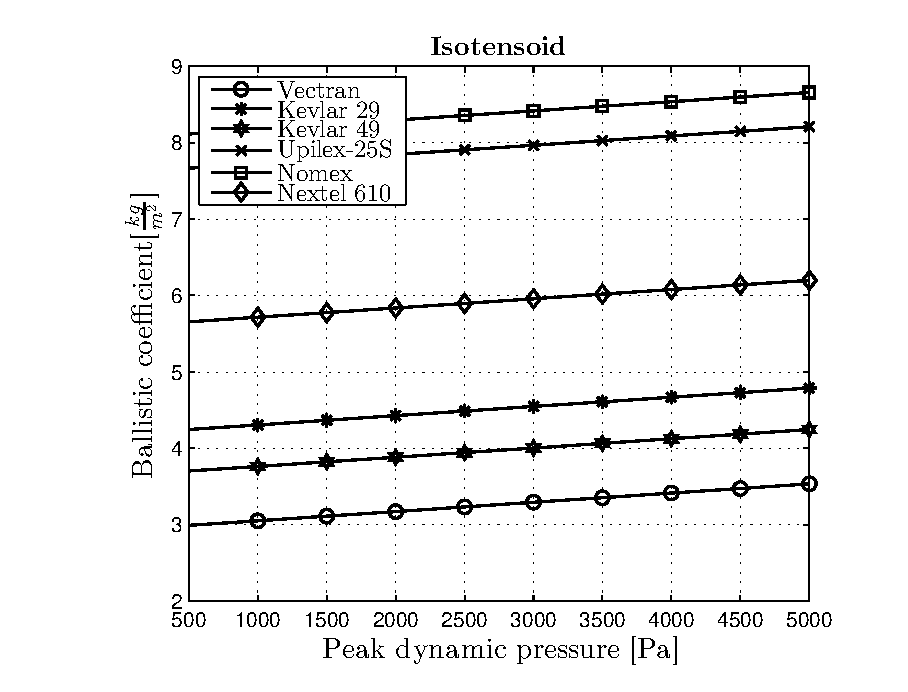
\includegraphics[width = 0.55\textwidth]{Figure/ISO_mat.eps}
\caption{Decelerator ballistic coefficient versus peak dynamic pressure for various materials of the isotensoid configuration, for \gls{sym:CD} = 1.5 [-] and a deployed diameter of 12 [m]}
\label{fig:ISO_mat}
\end{figure}
From Figure \ref{fig:ISO_mat}, it may be observed that the isotensoid configuration has the lowest ballistic coefficient (as per the tool implemented from Ref.\cite{Anderson1969}), and thereby the lowest mass, in case Vectran is used. Kevlar 49 and Kevlar 29 follow up, with ballistic coefficients approximately 30 $\%$ respectively 40 $\%$ higher than that obtained using Vectran. Use of Nextel 610, Upilex-25S and Nomex results in significantly higher ballistic coefficients. In case of Nomex, the ballistic coefficient is over 250 $\%$ higher than that in case of Vectran. Over the range of peak dynamic pressure considered, these mass performance differences are maintained. 

\begin{figure}[H]
\hspace{-35mm}
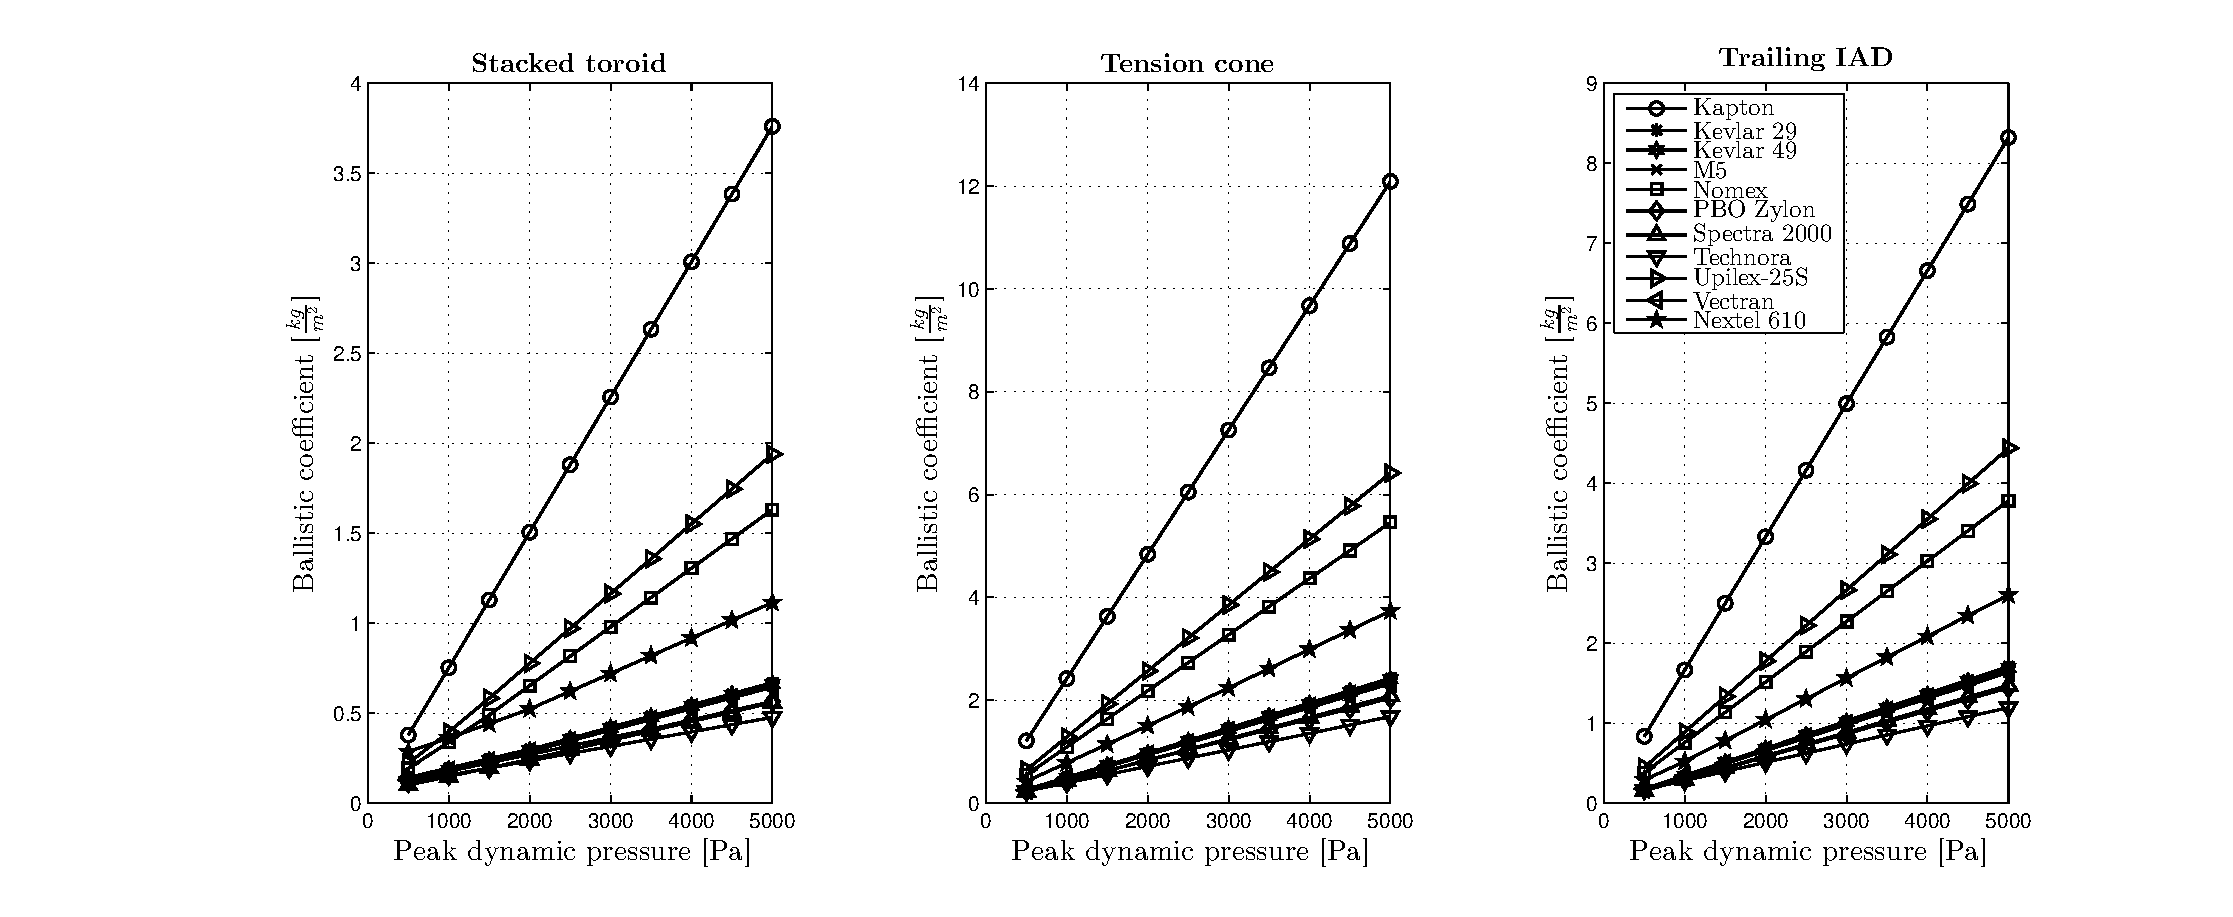
\includegraphics[width = 1.35\textwidth]{Figure/all_mat.eps}
\caption{Decelerator ballistic coefficient versus peak dynamic pressure for various materials of the stacked toroid, tension cone and trailing ballute configurations for \gls{sym:CD}= 1.5 [-] and a deployed diameter of 12 [m]}
\label{fig:all_mat}
\end{figure}

The ballistic coefficients of stacked toroid, tension cone and trailing \gls{iad}/ballute configurations, as produced by the tool implemented from Ref.\cite{Samareh2011}, are displayed in Figure \ref{fig:all_mat}. The sub-plots in this figure confirm that Nextel 610, Upilex-25S and Nomex perform worst in terms of effecting a low mass and thereby \gls{bc}. Kapton, however, is shown to perform worse still. The other materials, Kevlar 29, Kevlar 49, M5, PBO Zylon, Vectran, Spectra 2000 and Technora perform best and yield similar ballistic coefficients. While there are still differences between the mass performance, differences remain limited (in the order of 20-30 $\%$). In contrast to the isotensoid mass estimation, the estimation for the stacked toroid, tension cone and trailing ballute configurations has a stronger dependence on peak dynamic pressure: differences between materials are larger for an increasing peak dynamic pressure.

A combination of figures \ref{fig:ISO_mat} and \ref{fig:all_mat} yields that the best performance in terms of structural mass is achieved by using Technora, Spectra 2000 and PBO Zylon, followed closely upon by Kevlar 29, Kevlar 49 and Vectran. The former three are relatively new concepts, PBO Zylon the only one introduced in an \gls{iad} in IRVE-III \cite{Dillman2012}, in which it replaced the Kevlar (type unspecified) used in previous IRVE missions \cite{Lindell2006}. These observations are supported by the figures given by Miller et al \cite[p.7-p.8]{Miller2014}. 

For further design stages, this provides an indication of the effectiveness of certain materials. Their structural and thermal performance, however, remains to be investigated in the structural analysis and design phase following upon concept selection after the trade-off phase. 


